
%%%%%%%%%%%%%%%%%%%%%%%%%%%%%%%%%%%%%%%%%%%%%%%%%%%%%%%%%%%%%
%%%%%%%%%%%%%%%%%%%%%%%%%%%%%%%%%%%%%%%%%%%%%%%%%%%%%%%%%%%%%
%
%  %%%%%%%  %    %  %%%%%%  %%%%%%  %%%%%%%  %%%%%%%  %%%%%
%  %        %    %  %    %  %     %    %     %        %    %
%  %        %    %  %%%%%%  %     %    %     %        %    %
%  %        %%%%%%  %    %  %%%%%%     %     %%%%%    %%%%%
%  %        %    %  %    %  %          %     %        %    %
%  %%%%%%%  %    %  %    %  %          %     %%%%%%%  %     %
%
%%%%%%%%%%%%%%%%%%%%%%%%%%%%%%%%%%%%%%%%%%%%%%%%%%%%%%%%%%%%%
%%%%%%%%%%%%%%%%%%%%%%%%%%%%%%%%%%%%%%%%%%%%%%%%%%%%%%%%%%%%%

\chapter{Sheaves and Cosheaves in Sensor Networks}
\label{sec:sensors}

\begin{quote}
{\em``What strength, what art can then suffice, or what evasion bear him safe through the strict sentries and stations thick of angels watching round?''}
\begin{flushright} --- John Milton, Paradise Lost, Book II, Line 410~\cite{milton2008paradise} \end{flushright}
\end{quote}

In this section, we consider a candidate application of sheaves and cosheaves to problems in sensor networks. Section \ref{subsec:sensors} outlines some real-world  sensors as well as their mathematical abstraction. With this abstraction in hand, we consider in Section \ref{subsec:coverage} the classic problem of determining when a sensor network has completely covered a region. The introduction of time-dependent sensor networks necessitates the sheaf-theoretic approach, despite the fact that it is unwieldy in its most general form.

In Section \ref{subsec:intruder_bcs} we attempt to ``linearize'' the sheaves and cosheaves used in studying sensor networks in the hope that sheaf cohomology and cosheaf homology will give us an obstruction-theoretic approach to sensing. An approach of Henry Adams is considered in Section \ref{subsubsec:ttt_bcs}, as well as his counter-example to that approach. By using cosheaf-theoretic reasoning, we give a principled explanation for why this approach fails in Proposition \ref{prop:long_bcs}. An approach of the author and Robert Ghrist is then considered in Section~\ref{subsubsec:lss_bcs}. This approach succeeds where the previous approach fails, but it too suffers from giving false positives, as the example in Proposition \ref{prop:mobile_d4} shows. The example constructed there, which is joint with David Lipsky, uses one of the 12 indecomposable representations of the Dynkin diagram $D_4$.

Finally, a linear model for multi-modal sensing is presented in Section \ref{subsec:multi_modal}. It was there that the author realized the necessity of using indecomposables to interpret sheaf cohomology computations. A delightful examination of the act of sensing in Section \ref{subsubsec:deep_sense} shows how sheaves and cosheaves work in tandem. Theorem \ref{thm:les_sensing} uses a long exact sequence in sheaf cohomology to obtain a forcing result in multi-modal sensing. Finally, the role of higher-dimensional barcodes in multi-modal sensing is considered in Section \ref{subsubsec:evasion_bcs}. 

\section{A Brief Introduction to Sensors}
\label{subsec:sensors}\index{sensors}

Sensors are devices with delimited purview. They can measure certain properties and interact with occupants of a particular part of space-time. Examples abound in our world and they operate via differing modalities. Here are a few examples:

\begin{ex}[Sight]
	Our eyes are highly tuned sensors that can detect photons with certain frequencies (visible light and colors) and their spatial range can be on the order of kilometers. Some man-made satellites orbiting the Earth have cameras with a greater spatial resolution and frequency response --- they help us navigate by providing detailed pictures of roads, weather and climate. Eyes and satellites have a large scale and are very expensive. Cheaper sensors which can read only very coarse changes in light levels are found in our traffic lights, door ways and bathrooms.
\end{ex}

\begin{ex}[Weight and Pressure]
	Buried in roads or placed under door mats are sensors designed to respond to pressure. These open doors or gates or initiate changes in traffic signals. Some are more passive and merely collect data. A cable as thick as a thumb can be laid across a road and will record when something heavy (like a car) drives over it. Two spikes in pressure close in time indicate when a car's front and back wheels respectively drove over the cable. From this city officials can measure how fast cars are going as well as density and total volume of traffic.
\end{ex}

\begin{ex}[Radio Frequency ID]
	Some readers probably have a university card, or building card, that grants them access through locked doors merely by tapping on a sensor. Commuters drive cars equipped with sensors that allow them to pass through tolls without stopping. Some scientists tag animals to study a species' habits and movements. In all these cases, the sensor or the tag emits an electromagnetic field with limited spatial range (a few centimeters, meters, or kilometers) and only when inside this range is a tuned circuit thereby completed, connecting the sensors (card reader, toll booth, etc.) with the things being sensed (ID card, tag, etc.).
\end{ex}

Although the physical mechanisms that allow each of these sensors to sense is different, there are some broad commonalities: spatially localized sensors return data in the presence of certain occupants, which we call \textbf{intruders}. 

\section{The Coverage Problem: Static and Mobile}
\label{subsec:coverage}

The way we model sensors is to first identify the physical domain where the sensing is taking place --- a two-dimensional Euclidean plane could represent the floor of a building --- and we represent the sensors spatially via their support --- a door mat with pressure sensors would be a rectangle in the plane. Or we could think of the field of view of a camera in a ceiling pointed directly down as a disk in the plane. 

For the moment we ignore the type of data a sensor reports (we'll take that up later when we work with sheaves and cosheaves) and instead we consider the \textbf{coverage problem}: Given a collection of sensors distributed in a physical domain $D$, can we monitor the entire region without gaps?

\begin{figure}
\centering
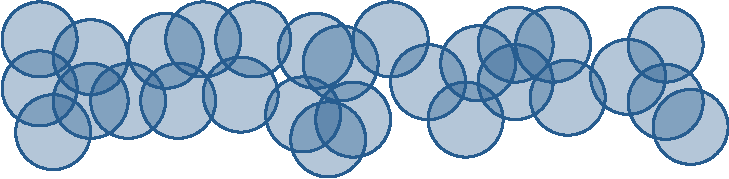
\includegraphics[width=\textwidth]{sensors.pdf}
\caption{Sensors Distributed in a Plane}
\label{fig:sensors5in}
\end{figure}

If we have good knowledge of the sensors which live on the boundary of our region, then we can, following the work of Vin de Silva and Robert Ghrist~\cite{VdSRG}, give a certificate of coverage using relative homology. However, we frame this question using sheaves of sets instead, so as to better handle the time-dependent scenario.\footnote{The author would like to thank Gunnar Carlsson and Rob Ghrist for their insights here.}

\begin{defn}\index{intruder problem}
Let $D$ be a spatial region of interest and denote by $D\times[0,1]$ a region of space-time. This carries with it a map that keeps track of time via projection onto the second factor, i.e. $\pi_2:D\times [0,1]\to[0,1]$. We assume that $D$ can be given a cell structure so that the sensors' \textbf{coverage region} $S\subset D\times [0,1]$ and the \textbf{evasion region} $E:=S^c$ can be written as the union of cells. To study the \textbf{intruder problem} is to analyze the associated sheaf of sections of the map $\pi:=\pi_2|_E :E\to [0,1]$, which we assume can be made cellular. Saying that there is an \textbf{evasion path} is to say there is a global section of this map, i.e. a $s:[0,1]\to E$ such that $\pi\circ s=\id$.
\end{defn}

\begin{figure}
\centering
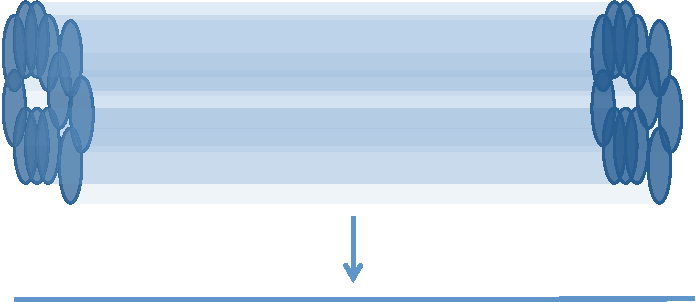
\includegraphics[width=\textwidth]{coverage_section.pdf}
\caption{The Space-Time Perspective}
\label{fig:coverage_section}
\end{figure}

\begin{ex}
For the situation depicted in Figure \ref{fig:coverage_section}, the intruder problem has a clear answer. An intruder can evade detection by residing in either one of the two holes present. Picking a point and then resting there for all time determines a global section of the time projection map. 
\end{ex}

It should be clear that our sheaf-theoretic question is equivalent to a much simpler one: ``Is the complement of the sensed region (the uncovered region) in $D$ non-empty?'' Thinking in terms of sheaves, at this point, buys us nothing. 

Where sheaves begin to offer a hint of leverage is in the time-dependent scenario. Here we imagine the sensors can move around in our domain $D$. Now it is possible that the sensed region $S$ does not look like a product of space and time.
 
\begin{figure}
\begin{center}
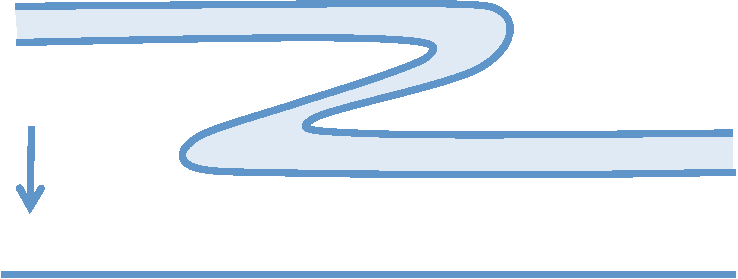
\includegraphics[width=.7\textwidth]{evade_sketch.pdf}
\caption{Mobile Sensor Network}
\label{fig:mobile_s}
\end{center}
\end{figure}

\begin{ex}
In Figure \ref{fig:mobile_s} we imagine that there is a one-dimensional environment of interest that sits vertically over each point on the time axis. Between the black lines is a region that is currently being unmonitored. To begin there is only one connected component of the unmonitored region. As time marches forward to the right a second connected component of the unmonitored region opens up, followed shortly by a third. Two of these three merge and then disappear leaving only one component of unmonitored territory.

In this case the non-existence of an evasion path is clear: no intruder could have gone undetected without time-traveling. This corresponds to the ready-seen fact that this map has no section, i.e. there does not exist a map $s:[0,1]\to E$ such that $\pi\circ s=\id$.
\end{ex}

What is the purpose of considering sheaves at all? If we can stare at the drawing and detect whether a section exists or not, why bother with high-flown machinery? However, what is easily seen in toy examples, can quickly become unmanageable. The only mathematics that formalizes intuition about sections is sheaf theory and moreover, once formalized using cellular sheaves, it can be programmed on a computer. 

However, there is a disadvantage with using sheaves of sets. We'd like to be able to calculate an obstruction that would certify whether a global section exists or not. One of the stated purposes of using sheaf cohomology is to provide such a calculable obstruction. Unfortunately, cohomology requires the linear structure of vector spaces, which we do not have here. In the next section we consider what happens when we na\"ively ``linearize'' the sheaf of sections of a map.

\section{Intruders and Barcodes}
\label{subsec:intruder_bcs}

In this section, we use cellular sheaves and cosheaves to analyze the intruder problem in the time-dependent case. We assume that the time projection map $\pi$ is cellular in order to take advantage of the functors in Section \ref{sec:maps}.
By putting a sheaf or cosheaf on the evasion region and pushing forward along $\pi$, we reduce the intruder problem to one dimension where we can use the barcode perspective of Section~\ref{sec:barcodes}. There are two main approaches, both of which have their drawbacks:

\begin{itemize}\index{intruder problem!approaches to}
	\item One approach is to study the homology of the evasion region at each moment in time $\pi^{-1}(t)$. By Theorem~\ref{thm:strat_maps}, this determines a cellular cosheaf.
	\item The second approach is to linearize the space of sections of the map $\pi$. To make the space of sections finite, we pass to the Reeb graph of the evasion region. This determines a cellular sheaf and stays true to the original intruder problem.
\end{itemize}

\subsection{Tracking the Topology over Time}
\label{subsubsec:ttt_bcs}

\begin{figure}
\begin{center}
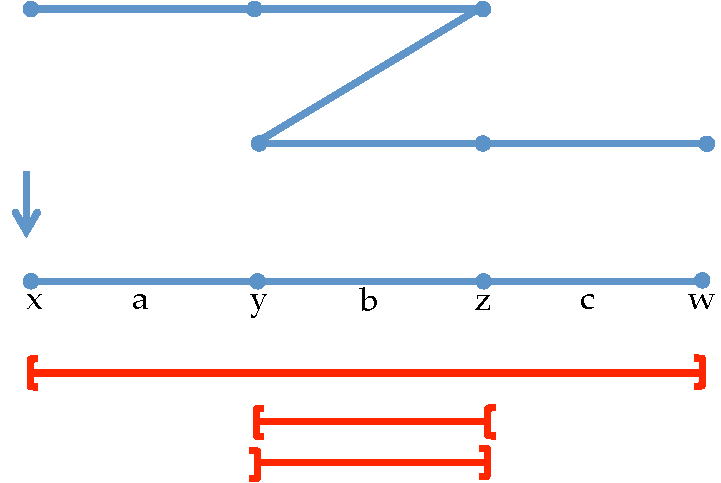
\includegraphics[width=.7\textwidth]{mobile_reeb_bc_new.pdf}
\caption{Mobile Sensor Network}
\label{fig:mobile_reeb_bc}
\end{center}
\end{figure}

To simplify the topology, we focus on the Reeb graph version of Figure \ref{fig:mobile_s}. This is drawn and labeled in Figure \ref{fig:mobile_reeb_bc}. Since everything is occurring in two-dimensional space-time, the only interesting homological invariant of the fiber is $H_0$. Studying this is equivalent to studying the pushforward cosheaf $\hF:=\pi_*\hat{k}_E$. In the parlance of~\cite{zigzag}, this is simply a zigzag module of the following form:
\[
	\xymatrix{\hF(x) & \ar[l]_{r_{x,a}} \hF(a) \ar[r]^{r_{y,a}} & \hF(y) & \ar[l]_{r_{y,b}} \hF(b) \ar[r]^{r_{z,b}} & \hF(z) & \ar[l]_{r_{z,c}} \hF(c) \ar[r]^{r_{w,c}} & \hF(w) \\
	k_x & \ar[l] k_a \ar[r]^{} & k^2_y & \ar[l] k^3_b \ar[r] & k^2_z & \ar[l] k_c \ar[r] & k_w}
\]

If we choose for each cell in $[0,1]$ the ordered basis given by the top down ordering on the page of the cells in the fiber we get the following matrix representations of the extension maps:
\[
	r_{y,a}=\begin{bmatrix} 1\\ 0\end{bmatrix} \quad r_{y,b}=\begin{bmatrix} 1 & 0 & 0\\ 0 & 1 & 1\end{bmatrix} \quad r_{z,b}=\begin{bmatrix} 1 & 1 & 0\\ 0 & 0 & 1\end{bmatrix} \quad r_{x,c}=\begin{bmatrix} 0\\ 1\end{bmatrix}
\]
We can decompose this cosheaf into indecomposables simply by performing the correct change of basis:
\[
	\begin{bmatrix} y_1'= y_1 \\ y'_2=y_1-y_2\end{bmatrix} \qquad \begin{bmatrix} b_1'= b_1-b_2+b_3 \\ b'_2=b_1-b_2 \\ b_3'=b_2-b_3 \end{bmatrix} \qquad \begin{bmatrix} z_1'= z_2 \\ z'_2=z_1-z_2\end{bmatrix}
\]
The reader should match the resulting indecomposables with the barcodes drawn in Figure \ref{fig:mobile_reeb_bc}.
\[
\xymatrix{k_x & \ar[l] k_a \ar[r]^{} & k_{y_1'} & \ar[l] k_{b_1'} \ar[r] & k_{z_1'} & \ar[l] k_c \ar[r] & k_w \\
0 & \ar[l] 0 \ar[r] & k_{y_2'} & \ar[l] k_{b_2'} \ar[r] & 0 & \ar[l] 0 \ar[r] & 0 \\
0 & \ar[l] 0 \ar[r] & 0 & \ar[l] k_{b_3'} \ar[r] & k_{z_2'} & \ar[l] 0 \ar[r] & 0
}
\]

The presence of a long barcode may seem surprising. It indicates that there is a connected component of the evasion region that persists for all time. The following proposition explains why this long barcode must exist.

\begin{prop}\label{prop:long_bcs}
	Suppose $E\subset D\times [0,1]$ is a compact connected evasion region such that $\pi=\pi_2|E$ is surjective, i.e. there is at each point in time somewhere an intruder can evade detection, then the Remak decomposition of $\pi_*\hat{k}_E$ must have a barcode that stretches the length of $[0,1]$.
\end{prop}
\begin{proof}
	The proof starts with the easy observation that if $f:Y\to X$ is a continuous map and $\hG$ is a cosheaf on $Y$, then we have that $H_0(Y;\hG)\cong H_0(X;f_*\hG)$. This follows from the commutativity of the following diagrams and functoriality of pushforward.
	\[
		\xymatrix{Y \ar[rr]^f \ar[rd]^p & & X \ar[ld]_p \\ & \star &} \quad \xymatrix{\hG \ar[rr]^{f_*} \ar[rd]^{p_*} & & f_*\hG \ar[ld]_{p_*} \\ & p_*\hG\cong (p\circ f)_*\hG &}
	\]
	Setting $Y=E$, $X=[0,1]$, $f=\pi$ and $\hG=\hat{k}_E$, we can use the fact that $E$ is connected to get that $p_*\hat{k}_E\cong H_0(E;\hat{k}_E)\cong k$. We know that any (co)sheaf over $[0,1]$ can be written as a direct sum of constant (co)sheaves supported on barcodes.
	\[
		\pi_*\hat{k}_E\cong \hat{k}_{B_1}\oplus \cdots \oplus \hat{k}_{B_n} \qquad \qquad \mathrm{and}
	\]
	 Now we combine this with the fact that homology commutes with direct sums.
	\[
		k\cong H_0(E;\hat{k}_E)\cong H_0([0,1];\pi_*\hat{k}_E)\cong \bigoplus_i  H_0([0,1];\hat{k}_{B_i})\cong \bigoplus_i  H^{BM}_0(B_i) .
	\]
	Consequently, there can be only one closed barcode. We argue that this unique closed barcode must have support on all of $[0,1]$. Since we know that the constant section $1_E\in \Gamma(E;\hat{k}_X)$ has support on all of $E$, the pushforward section $\pi_*1_E$ that generates the closed barcode must have support on all of $[0,1]$, since $\pi$ is surjective.
\end{proof}

\begin{rmk}
	We have implicitly used sheaf-theoretic reasoning with $H^0$ taking the place of $H_0$. The argument about the support of the section is better expressed using stalks.
\end{rmk}

 As a consequence, we obtain a negative result, which is almost identical to a result of Henry Adams.

\begin{cor}
	Having a barcode associated to $\pi_*\hat{k}_E$ whose support is all of $[0,1]$ does not indicate the existence of an evasion path.
\end{cor}

\begin{rmk}
The above proof gives a cosheaf-theoretic explanation of why we shouldn't expect barcodes to detect the existence of an evasion path. Homology of the evasion region is not sensitive to its embedding, thus a long barcode will appear even if it is embedded in a way that would require an intruder to time travel. In this sense, Corollary \ref{cor:barcode_homology} can be interpreted as a stability result: although half-open barcodes can pop in and out of existence, based on the embedding, there must always be one and only one closed barcode.
\end{rmk}
  

\subsection{Linearizing the Sheaf of Sections}
\label{subsubsec:lss_bcs}

\begin{figure}[ht]
\begin{center}
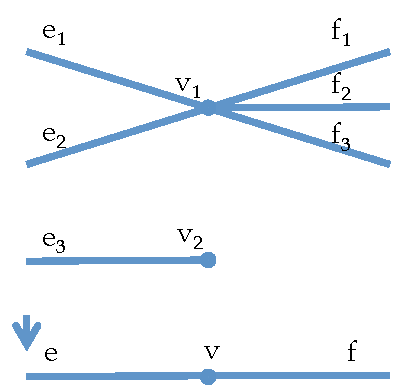
\includegraphics[width=.5\textwidth]{route_stack_new.pdf}
\caption{Sheaf of All Possible Evasion Paths}
\label{fig:route_stack}
\end{center}
\end{figure}

In light of the inability of the pushforward cosheaf $\pi_*\hat{k}_E$ to distinguish when an evasion path exists or not, we return to the original sheaf-theoretic formulation of the intruder problem. To make the sheaf of sections finite enough to work with, we take the Reeb graph of the map $\pi:E\to[0,1]$. From this setup, we can extract a cellular map of 1-dimensional cell complexes, normally called $\tilde{\pi}:R(\pi)\to [0,1]$, but we will abuse notation and assume that our input $\pi: E\to [0,1]$ is already a Reeb graph.

By picking a directionality of $[0,1]$ we can endow $E$ with the structure of a directed graph. On this directed graph we can define the following cellular sheaf, which is meant to pushforward to a linear model of the sheaf of sections. It is very closely related\footnote{In a sense, the sheaf defined here gives all possible codings. It approximates a ``stack'' of network coding sheaves.} to the network coding sheaves defined in Section \ref{sec:nc_coding}.

\begin{defn}
	Let $X$ be an acyclic directed graph. We define a cellular sheaf $G$ that assigns to an edge the one-dimensional vector space $k$ and assigns to a vertex the space freely generated by all possible directed routings through that vertex. 
	
	We allow special treatment to a subset of sources $S$ and sinks $T$, where we allow $G(v)=k^{\out(v)}$ for $v\in S$ and $G(v)=k^{\inn(v)}$ for $v\in T$. All other sources and sinks get the zero vector space. The restriction mappings send a routing to the edges that participate in that routing.	
\end{defn}

\begin{ex}
For a concrete example, where we focus on a small part of a graph, consider the graph in Figure \ref{fig:route_stack}. The definition of the sheaf $G$ makes
\[
	G(v_1)=<e_i\otimes f_j \, | \, i=1,2; \,j=1,2,3>\cong k^6 \qquad \rho_{e_i,v_1}(e_j\otimes f_k)=\delta_{ij} \quad \rho_{f_j,v_1}(e_i\otimes f_k)=\delta_{jk} 
\]
and we choose to make $G(v_2)=0$. The reason we have decided to set $G(v_2)=0$ comes from the extra information of the projection map to $[0,1]$. We call such a vertex an \textbf{internal} source or sink. In the context of the intruder problem, an internal source represents an impossible entry point for an intruder. If we push the sheaf $G$ along the projection map $\pi$ we then get the following assignments of data:
\[
	\pi_*G(e)\cong<e_1,e_2,e_3> \quad \pi_*G\cong G(v_1) \quad \pi_*G(f)=<f_1,f_2,f_3>
\]
\end{ex}

\begin{figure}
\begin{center}
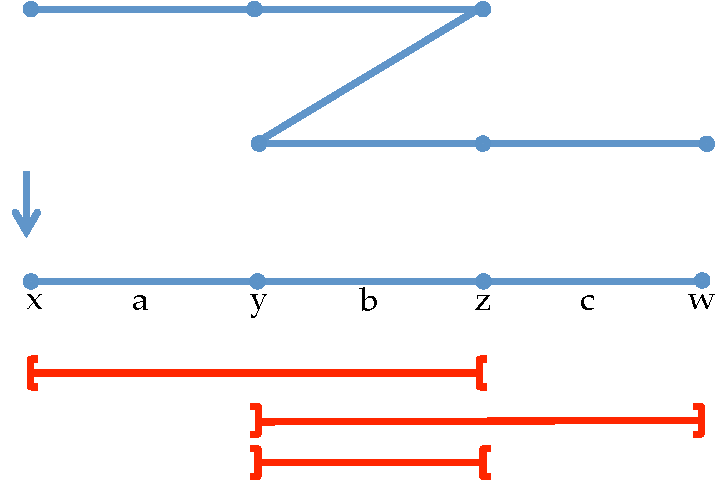
\includegraphics[width=.7\textwidth]{evade_sec_bc_new.pdf}
\caption{Linearized Sheaf of Sections}
\label{fig:evade_sec_bc}
\end{center}
\end{figure}

\begin{ex}
Let us consider the example drawn in Figure \ref{fig:evade_sec_bc}, but now with the sheaf just defined. We set $F=\pi_*G$, whose values are below:

\[
	\xymatrix{F(x) \ar[r]^{\rho_{a,x}} & F(a) & \ar[l]_{\rho_{a,y}}  F(y) \ar[r]^{\rho_{b,y}} & F(b) & \ar[l]_{\rho_{b,z}} F(z) \ar[r]^{\rho_{c,z}} & F(c) & \ar[l]_{\rho_{c,w}} F(w) \\
	k_x  \ar[r] & k_a & \ar[l] k_y \ar[r] &  k^3_b & \ar[l] k_z \ar[r] &  k_c & \ar[l]  k_w}
\]
The two restriction maps of any interest include into the top section and the bottom section, respectively.
\[
	\rho_{b,y}=\begin{bmatrix}1 \\0\\0\end{bmatrix} \qquad \rho_{b,z}=\begin{bmatrix}0 \\0\\1\end{bmatrix}
\]
Without a change of basis one can see that this sheaf splits as the direct sum of indecomposables, whose barcodes are drawn in Figure \ref{fig:evade_sec_bc}.
\end{ex}

The previous example offers a glimmer of hope. No intruder can evade detection and the absence of a long barcode reflects that. Moreover, the sheaf cohomology computation shows $H^0([0,1];F)\cong 0$, which would be a promising shortcut to computing barcodes. Alas, the linearized sheaf of sections fairs no better than the cosheaf of components. Here we provide a counterexample, joint with Dave Lipsky, to either of the hopes that non-zero $H^0([0,1];F)$ or a long barcode provides an if and only if criterion for the existence of an evasion path.

\begin{figure}
\begin{center}
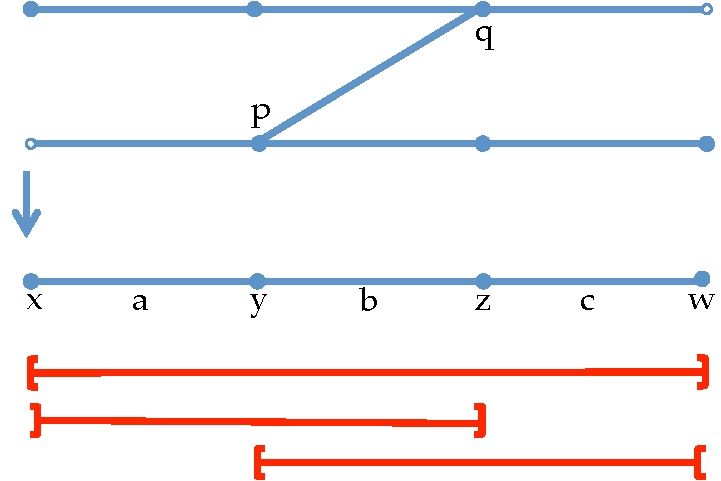
\includegraphics[width=.7\textwidth]{mobile_d4_1.pdf}
\caption{Counterexample for the Linearized Sheaf of Sections}
\label{fig:mobile_d4}
\end{center}
\end{figure}

\begin{prop}\label{prop:mobile_d4}
	Although it is true that the existence of an evasion path implies the existence of a long barcode (and thus $H^0([0,1];F)\neq 0$) it is not true that having a long barcode (or $H^0([0,1];F)\neq 0$, which is a weaker condition) implies the existence of an evasion path.
\end{prop}
\begin{proof}
	In Figure \ref{fig:mobile_d4} we have drawn the counter-example, which we now explain. The component coming into $p$ appears immediately after time $0$, so it is impossible for an intruder to enter there. Similarly, there is a component leaving from $q$ that closes up right before time $1$. The pushforward sheaf then takes the following form
	\[
		\xymatrix{	k_x  \ar[r] & k^2_a & \ar[l] k^3_y \ar[r] &  k^3_b & \ar[l] k^3_z \ar[r] &  k^2_c & \ar[l]  k_w}
	\]
	The maps from $F(y)$ and $F(z)$ to $F(b)$ are the identity maps. The two maps that require some inspection are built out of a projection and a trace map.
	\[
		\rho_{a,y}=\begin{bmatrix}1 & 0 & 0 \\0 & 1 & 1\end{bmatrix} \qquad \rho_{c,z}=\begin{bmatrix}1 & 1 & 0 \\0 & 0 & 1\end{bmatrix}.
	\]
	The change of basis required to obtain the desired Remak decomposition indicated by the barcodes is not so easily seen. The interval decomposition algorithm outlined in~\cite{zigzag} provides a sure-fire method of obtaining it. It is left to the reader to verify the the barcodes in Figure \ref{fig:mobile_d4}.
	
	Instead, we give a sheaf-theoretic justification for the existence of a long barcode. There is a unique non-zero global section of $G$ and it is supported everywhere except on the prong incoming to $p$ and outgoing from $q$. Explicitly, it comes from choosing a compatible kernel for the restriction matrices $\rho_{a,y}$ and $\rho_{c,z}$. At $q$ the routing through the top path is annihilated by the ``negative'' of the routing through the bottom path; it is as if two intruders are traveling with opposite charges. As a consequence, its support surjects onto all of $[0,1]$. Since $H^0([0,1];F)\cong k$ we can infer the existence of one closed barcode, and because this section has global support, the barcode must be long.
\end{proof}

\begin{rmk}[Dynkin Diagrams and Stalks]
	Recall that $F:=\pi_* G$. Consider the sheaf $G$ implied by Figure \ref{fig:mobile_d4}. When restricted to the open stars at $p$ and $q$ separately $G$ is equivalent to one of the 12 indecomposable representations of the Dynkin diagram $D_4$; see~\cite{etingof_rep}, p. 83. Since the open stars intersect, one can show that the entire sheaf $G$ on $E$ is indecomposable. This cannot be used directly to show that a long barcode must exist. The pushforward of an indecomposable representation is not necessarily indecomposable. However, the argument using stalks indicates that some sections (subrepresentations), must have global support.
\end{rmk}

\section{Multi-Modal Sensing}
\label{subsec:multi_modal}\index{sensors!multi-modal}

In this section we will explore the following cartoon for multi-modal sensing:

\begin{itemize}
	\item We have a region $W$ thought of as a topological space that is tame enough to be triangulated. This space is populated by agents of interest and sensors.
	\item There is a vector space of properties $k^n$, usually $\RR^n$ or $\CC^n$, and every intruder is tagged with an unchanging \textbf{property vector} $v\in k^n$. These property vectors might record colors (which we pretend has a linear structure), sounds, thermal signatures or, in the context of wireless network data, a unique wireless SSID (we imagine scaling corresponds to the strength of the signal). In future applications, $k$ may be a ring that stores data, just as $\ZZ$ is used to record counts and $\ZZ^n$ records counts of different types of targets.
	\item There are sensors who monitor subspaces of $k^n$ and subspaces of $X$. ``Monitors'' means explicitly that a sensor $i$ with support $V_i\subset X$ has attached to it a subspace of the vector space dual to property space, i.e. $S_i\subset k^{n*}$. For simplicity, we assume that $S_i=\mathrm{span}\{\xi_i\}=:<\xi_i>$. The act of sensing corresponds to taking a property vector $v\in k^n$ and returning a number $\xi_i(v)$ that records the strength of the detection. Outside of the sensor's support $V_i$, the sensor must return zero on every vector. In the overlap of two sensors' supports, the vector space that is sensed is the internal direct sum.
\end{itemize}

This cartoon specifically suggests the use of constructible sheaves and cosheaves as a model. Because the roles of sensors and intruders are formally dual, we will have to use \emph{both} sheaves and cosheaves. Understanding the formal properties of sensing and evasion will lead us naturally to some long-exact sequences in cohomology, which will necessitate the introduction of barcodes to understand these results. 

\begin{figure}
\centering
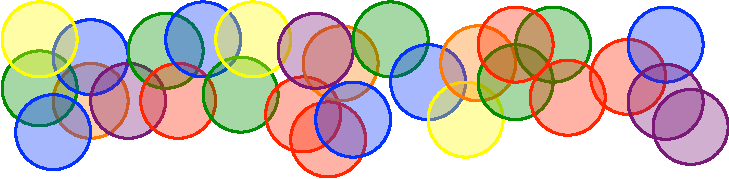
\includegraphics[width=\textwidth]{sensors_color.pdf}
\caption{Multi-Modal Sensors Distributed in a Plane}
\label{fig:sensors5in_color}
\end{figure}

We are going to work with a simplified version of the above cartoon. To detach ourselves from an embedding of the sensors into $W$, we will use the \v{C}ech nerve associated to the sensors supports. This will provide us with a simplicial complex $X$ and this where we will define sheaves and cosheaves. Since we can only analyze the intruder problem inside sensor's support, we call this a \textbf{relative intruder problem}. Working strictly inside the coverage region will introduce counter-intuitive results, such as Claim \ref{clm:no_sections}. Nevertheless, this setup is a prototype for future applications of sheaves and cosheaves to multi-modal sensing.

\subsection{A Deeper Look at Sensing}
\label{subsubsec:deep_sense}

Let us investigate a little more deeply the picture of multi-modal sensing presented to us in the above cartoon. In Figure \ref{fig:rg_sense}, we consider a situation where we have a sensor capable of detecting ``red'' properties and a sensor capable of detecting ``green'' properties.\footnote{We use scare quotes to indicate that the terms can be substituted for whatever application is of interest.}

On the nerve of the sensor cover, the organizing diagram of vector spaces is clear.
\[
	<r^*>\hookrightarrow <r^*,g^*> \hookleftarrow <g^*> \qquad k \hookrightarrow k^2 \hookleftarrow k
\]
The direction of the arrows indicates that a cellular sheaf is best used to collate sensing abilities. However, the diagram of abstract vector spaces on the right has no way of telling whether an individual copy of $k$ should correspond to $<r^*>$ or $<g^*>$ or $<b^*>$. Such a distinction requires that we embed our sensing sheaf into a global system of coordinates $(k^n)^*_X$. This motivates the following definition.

\begin{defn}[Sensing Sheaf]\index{sensing sheaf}\index{sheaf!sensing}
	Suppose we have a multi-modal sensor network distributed in a space $W$. Form the nerve given by the intersections of the sensors' supports and call this simplicial complex $X$. We define a \textbf{sensing sheaf} $F$ by assigning to each vertex $v$ in $X$ the subspace $S_v\subset (k^n)^{*}$. Over higher simplices $\sigma$ we assign the following vector spaces and use the natural inclusions for the maps internal to the sheaf:
	\[
		F(\sigma)=S_{v_0}+\cdots + S_{v_n} \qquad F(\sigma)\hookrightarrow F(\tau) \quad \sigma\leq \tau.
	\]
	Here we have used the internal sum of subspaces to reflect the fact there may be dependencies. The internal sum is only defined in the presence of an ambient space, thus part of the data of a sensing sheaf is an embedding into the constant sheaf of all sensing abilities:
	\[
		\iota_F: F \hookrightarrow k^{n*}_X.
	\]
\end{defn}

\begin{figure}
\centering
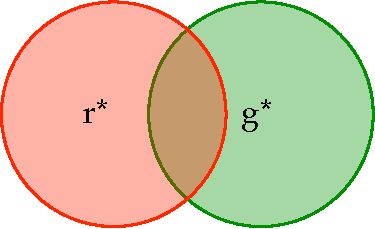
\includegraphics[width=.5\textwidth]{rg_sense.pdf}
\caption{Two Multi-Modal Sensors}
\label{fig:rg_sense}
\end{figure}

Now suppose we have an intruder, which we imagine as a point in the union of the red and green sensors in Figure \ref{fig:rg_sense}. The intruder has a property vector $v\in k^n$ that lists its various attributes, its colors in this example. What number does the sensor return while the intruder is in the red sensor's domain? By design, it is $r^*(v)$, the contraction of the red co-vector and the property vector $v$. If $k^n=k^3=<v_r,v_g,v_b>$ is a three dimensional property space spanned by the attributes ``red,'' ``green,'' and ``blue,'' equipping it with the standard Euclidean inner product allows us represent this measurement by the matrix product
\[
	r^*(v)=\begin{bmatrix} 1 & 0 & 0\end{bmatrix}\begin{bmatrix} v_r \\ v_g \\ v_b\end{bmatrix}=v_r
\]

However, if the sensors can collaborate and share information, then we can store together the observations when the intruder is in the intersection of the red and green sensors' support.
\[
	\begin{bmatrix} r^*(v) \\ g^*(v)\end{bmatrix}=\begin{bmatrix} 1 & 0 & 0 \\ 0 & 1 & 0\end{bmatrix}\begin{bmatrix} v_r \\ v_g \\ v_b\end{bmatrix}=\begin{bmatrix} v_r \\ v_g\end{bmatrix}
\]
We can package these measurements into a cellular cosheaf, where two observations are the same modulo the properties unobserved by the sensors.
\[
	<r> \leftarrow <r,g> \rightarrow <g> \qquad \frac{k^3}{<g,b>} \leftarrow \frac{k^3}{<b>} \rightarrow \frac{k^3}{<r,b>}
\]

One should note that the right side gives an equivalent formulation for the \textbf{measurement cosheaf} of the Figure \ref{fig:rg_sense}. We have over each cell passed to the quotient space where the properties that are invisible to each of the sensors is treated as zero. In other words, the vectors produced by the process of measurement must naturally be considered modulo the unknown.

\begin{defn}[Evasion Co-Sheaf]\index{evasion cosheaf}\index{cosheaf!evasion}
	Given a sheaf $F$ whose restriction maps are inclusions, along with a fixed embedding into a locally constant sheaf of vector spaces $G$ (we take $G=k^{n*}_X$), we define the \textbf{annihilator cosheaf} $\widehat{Ann}(F)$ as follows:
	\begin{itemize}
		\item $\widehat{Ann}(F)(\sigma)=\{v^*\in G(\sigma)^{*}| v^*(\iota(w))=0\quad \forall w\in F(\sigma)\}$
		\item If $\sigma\subset\bar{\tau}$, then $r_{\sigma,\tau}:\widehat{Ann}(F)(\tau)\to \widehat{Ann}(F)(\sigma)$ is the inclusion.
	\end{itemize}
	When using the language of sensing sheaves, we will call $\widehat{Ann}(F)=:\hat{E}$ the \textbf{evasion cosheaf}.
\end{defn}

\begin{lem}\label{lem:evade_cok}
	Let $F$ be a sensing sheaf on $X$, then the evasion cosheaf is canonically identified as the linear dual of the cokernel of the embedding, that is to say that $\hat{E}\cong \hat{V}(\cok(\iota))$ in the diagram below.
	\[
		\xymatrix{0 \ar[r] & F \ar[r]^{\iota} \ar@{~>}[d] & G \ar[r]^{q} \ar@{~>}[d] & \cok(\iota) \ar[r] \ar@{~>}[d] & 0 \\
		0 & \ar[l] \hat{V}(F) & \ar[l] \hat{V}(G) & \ar[l] \hat{V}(\cok) & \ar[l] 0 }
	\]
\end{lem}
\begin{proof}
	Here we make use of the fact that for cellular sheaves, the cell-by-cell cokernel of the maps $\iota(\sigma):F(\sigma)\to G(\sigma)$ defines a sheaf. This is not always true for general sheaves. Reducing the argument to a cell-by-cell one, we have a short exact sequence of vector spaces
\[
	\xymatrix{0 \ar[r] & V \ar[r]^{\iota} & W \ar[r]^{q} & W/V \ar[r] & 0}
\]
where we can identify 
\[
Ann_W(V)=\{\varphi:W\to k\,|\,\varphi(v)=0\,\forall v\in V\}\cong (W/V)^{*}
\]
and of course all the restriction maps get sent to restriction maps
\[
\xymatrix{V_2 \ar[rd] & & (W/V_2)^{*} \ar[dd]\\
& W \ar[ru]\ar[rd] & \\
V_1 \ar[uu]\ar[ru] & & (W/V_1)^{*} .}
\]
\end{proof}

This identification of evasion cosheaves with the linear dual of a cokernel means that we can leverage a classical technique in studying the relative intruder problem. After all, to every short exact sequence of sheaves we get an induced long exact sequence of sheaf cohomology. In the context of multi-modal sensing this relates in a precise way the topology of the total covered region and the cohomology of the sensing and evasion sheaves. 

\begin{thm}[Sensing-Evasion Decomposition]\label{thm:les_sensing}\index{decomposition!sensing and evasion regions}
	Given a sensing sheaf of vector spaces $\iota:F\to G=\tilde{k}_X^{n^{*}}$ we obtain a long exact sequence of sheaf cohomology groups
\[
\xymatrix{
	            0\ar@{->}[r] & H^0(X;F)\ar@{->}[r] & H^0(X;k)^{\oplus n}\ar@{->}[r]
	                   & H^0(X;\cok(\iota)) \ar `r[d] `_l[lll] ^{\delta^0} `^d[dlll] `^r[dll] [dll] \\
	            & H^1(X;F)\ar@{->}[r] & \hspace{12pt}\cdots\hspace{12pt}\ar@{->}[r]
	                   & H^k(X;\cok(\iota)) \ar `r[d] `_l[lll] ^{\delta^k} `^d[dlll] `^r[dll] [dll] \\
	            &H^{k+1}(X;F)\ar@{->}[r] & H^{k+1}(X;k)^{\oplus n}\ar@{->}[r]
	                   & H^{n+1}(X;\cok(\iota)) \ar `r[d] `_l[lll] ^{\delta^{k+1}} `^d[dlll] `^r[dll] [dll] \\
	            & & \cdots &
	}
\]
Where $H^k(X;\cok(\iota))$ gets identified with the evasion co-sheaf's homology $H_k(X;\hat{E})$ via the linear duality functor, i.e. $V: \cok(\iota)) \rightsquigarrow E$.
\end{thm}
\begin{proof}
	The proof is immediate from standard homological algebra techniques.
\end{proof}

\subsection{Indecomposables, Evasion Sets, Generalized Barcodes}
\label{subsubsec:evasion_bcs}
One of the drawbacks of Theorem \ref{thm:les_sensing} is that we have no good interpretation of what the sheaf cohomology groups mean. Let's consider again Figure \ref{fig:rg_sense}, but this time let us focus only on the \v{C}ech complex and each of the three sheaves that appear in the short exact sequence. This is depicted in Figure \ref{fig:sense_bars}.

\begin{figure}
\centering
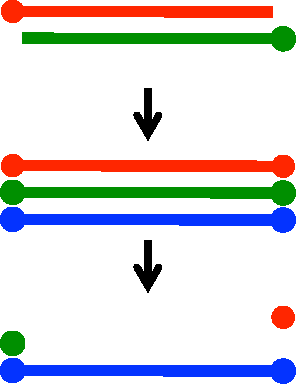
\includegraphics[width=.3\textwidth]{sense_bars.pdf}
\caption{Examining the Short Exact Sequence}
\label{fig:sense_bars}
\end{figure}

As can be clearly seen each sheaf appearing in the sequence is already written as a direct sum of indecomposables, which because the nerve is a one-simplex, look like barcodes. By using the observation $H^i([0,1];F)\cong \oplus H^i_c(B_i)$, which we have already made heavy use of, we can determine all the sheaf cohomology of interest for this example.

\begin{ex}[Red-Green Sensors]
	By inspection of the indecomposable presentations of the three sheaves $F$, $k^3_X$ and $\cok(\iota)$ in Figure \ref{fig:sense_bars} we see that
	\[
	H^i(X;F)\cong 0 \, i=0,1; \qquad H^0(X;k^3_X)\cong k^3 \qquad H^0(X;\cok(\iota))\cong H_0(X;\hat{E})\cong k^3 
 	\]
The interpretation of each of the three generators in the evasion cosheaf homology is that there is a connected component where red, green and blue can separately evade.
\end{ex}

\begin{defn}[Evasion and Detection Sets]
	Let $v\in k^n$ be a property vector and $F$ a sensing sheaf on $X$. Define the \textbf{evasion set} $E_v$ to be the set of points in $X$ where an intruder with property vector $v$ can go without being detected. Dually, call the set of points where $v$ can be detected the \textbf{detection set} $D_v$.
\end{defn}

Since we are working with cellular sheaves where individual sensors have support equal to the open star of their designated vertex in the simplicial complex $X$, thus the detection set $D_v$ is equal to the union of all the stars of the sensors that can see $v$, hence $D_v$ is an open union of cells. This proves the following lemma.

\begin{lem}
	For any property vector $v$, the evasion and detection sets form an open-closed decomposition of $X$, that is
	\[
		X=E_v\cup D_v \qquad E_v\cap D_v=\emptyset, \qquad E_v \,\, \mathrm{open}.
	\]
	When $X$ is compact this means that $E_v$ is compact as well.
\end{lem}

We record another easy lemma, connected to our desire to get an indecomposable presentation for our evasion cosheaves.

\begin{lem}
	Suppose that all sensors must pull their sensing capabilities from a fixed orthonormal basis of $k^{n*}$, say $v_1^*,\ldots, v_n^*$, then the evasion cosheaf splits as a direct sum decomposition of constant cosheaves supported on the evasion sets for $v_1,\ldots,v_n$
	\[
		\hat{E}\cong \hat{k}_{E_{v_1}}\oplus \cdots \oplus \hat{k}_{E_{v_n}}
	\]
	with the further observation that each $\hat{k}_{E_{v_i}}$ has a Remak decomposition as a sum of constant cosheaves supported on the components of $E_{v_i}$.
\end{lem}
\begin{proof}
	The fact that the sensor capabilities can only be chosen from a fixed orthonormal basis, implies that we can write the constant sheaf $k^{n*}_X$ as a direct sum of $k_X\oplus\cdots\oplus k_X$ where we think of each copy of $k_X$ as being the constant sheaf generated by $<v_i^*>$. As a consequence we get the following diagram
	\[
		\xymatrix{ & k_{D_{v_1}} \ar@{^{(}->}[r] & k_X \ar[dr]^{i_{v^*_1}} & \\
		F \ar[ur]^{\pi_{v^*_1}} \ar[dr]_{\pi_{v^*_n}} & \vdots & \vdots & k^{n*}_X \\
		  & k_{D_{v_n}} \ar@{^{(}->}[r] & k_X \ar[ur]_{i_{v^*_n}} & }
	\]
	Now we can use for each factor the following standard short exact sequence of sheaves
	\[
		\xymatrix{0 \ar[r] & k_{D_{v_i}} \ar[r] & k_X \ar[r] & k_{E_{v_i}} \ar[r] & 0}
	\]
	and thus the cokernel splits as a direct sum $\oplus_{i=1}^n k_{E_{v_i}}$.
\end{proof}	

The above lemma implies that in certain cases we can interpret the homology of the evasion cosheaf in terms of the topology of the evasion sets.

\begin{figure}
\centering
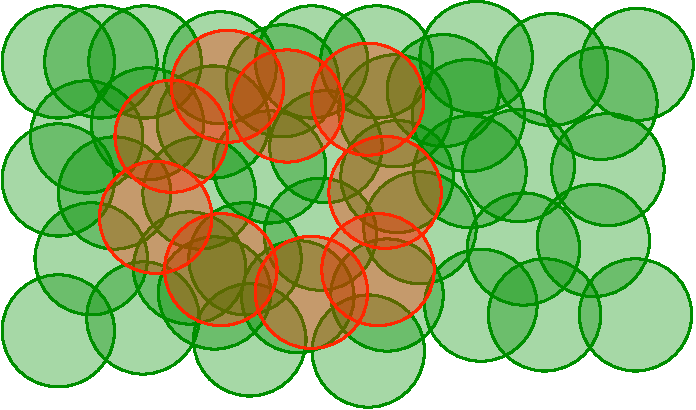
\includegraphics[width=.7\textwidth]{red_circle.pdf}
\caption{Short Exact Sequence}
\label{fig:red_circle}
\end{figure}

We have one more observation we'd like to leverage.

\begin{clm}\label{clm:no_sections}
	If sensor's abilities are pulled from a fixed orthonormal basis $v_1^*,\ldots, v_n^*$ and moreover the detection sets are not pairwise disjoint, then the sensing sheaf has no global sections.
\end{clm}
\begin{proof}
	This follows from the fact that if an edge is common to two different detection sets, then there can be no global sections since the following sheaf has no non-zero global sections
	\[
		<v_i^*> \hookrightarrow <v_i^*,v^*_j> \hookleftarrow <v_j^*>.
	\]
\end{proof}

For the example considered in Figure \ref{fig:red_circle} assume that the space of properties is two dimensional, spanned by red and green. Then the Theorem \ref{thm:les_sensing} provides the following forcing result
\[
 0 \to H^0_c(X;F)\cong 0 \to H^0_c(X;k^{2*}_X)\cong k^2 \to H^0_c(X;\cok) \to H^1_c(X;F)\cong k \to 0 
\]
which upon careful inspection reveals that the red evasion set must be disconnected.
